\chapter{Transformaties Combineren}
\label{hoofdstuk:ETT}

In dit hoofdstuk worden twee algoritmes behandeld die varianten zijn van elkaar. In beide algoritmes is het de bedoeling om een gegeven muziekstuk te transformeren tot een nieuw muziekstuk op zo een manier dat de totale consonantiescore zo hoog mogelijk is. Dit kan gebeuren door een aantal toegelaten operaties op het oorspronkelijke muziekstuk. Buiten de originele melodielijn zullen namelijk ook een aantal verschillende transformaties (zoals die beschreven zijn in onderdeel \ref{MT:afstand_vorige}) meegegeven worden aan het algoritme. Deze transformaties zullen door het algoritme gebruikt worden om het originele stuk te transformeren naar een nieuw stuk met een hogere consonantiescore (De score die gebruikt wordt is deze beschreven in onderdeel \ref{OBM:RPK}, volgens het `RPK-Model'). Voor elke noot van de melodielijn heeft het algoritme namelijk de keuze om ofwel de noot te behouden, ofwel deze te transformeren conform een van de transformaties die meegegeven werden aan het algoritme. Het algoritme dat hier voor zorgt wordt beschreven in onderdeel \ref{ETT:algo1}. In gedeelte \ref{ETT:algo2} wordt een algoritme beschreven dat eenzelfde doel heeft maar een extra voorwaarde opgelegd krijgt. Deze voorwaarde stelt dat als met een transformatie wilt toepassen, men telkens een minimum aantal opeenvolgende noten moet transformeren met dezelfde transformatie. \\
Het is belangrijk op te merken dat het opzet van deze algoritmen niet van die aard is deze daadwerkelijk te gaan gebruiken om muziekstukken te gaan cre\"eren die goed zullen klinken. Er wordt nadrukkelijk gebrobeerd om die melodielijn te vinden die een zo hoog mogelijke consonantiescore heeft volgens het RPK-model. Er werd echter reeds aangehaald dat muziekstukken met een zeer hoge consonantiescore niet goed klinken (veel dezelfde noten en heel kleine sprongen tussen opeenvolgende noten). Het opzet van deze algoritmen is om achteraf te kunnen bepalen hoe afhankelijk de consonantiescore zal zijn van het aantal transformaties dat toegepast wordt op het muziekstuk, wat de eventuele minimum transformatielengte als invloed heeft en hoe het aantal beschikbare transformaties de consonantiescore bepaalt.

\section{Beste sequentie}
\label{ETT:algo1}

\subsection{Doelstelling}
Het algoritme dat hier beschreven wordt is afhankelijk van twee parameters. Een eerste parameter is een originele melodielijn. De tweede parameter beschrijft een aantal transformaties (gedifini\"eerd zoals in onderdeel \ref{MT:afstand_vorige}), die gebruikt mogen worden door het algoritme. Het doel is nu om gebruik makend van enkel deze verschillende mogelijke transformaties de originele melodielijn te transformeren tot de nieuwe melodielijn die de hoogste consonantiescore oplevert. Hierbij heeft het algoritme voor elke noot in het muziekstuk twee mogelijke keuzes. Een eerste mogelijkheid is dat de noot niet getransformeerd wordt en identiek overgenomen wordt in de nieuwe melodielijn. De tweede mogelijkheid bestaat erin dat de noot ook getransformeerd mag worden, maar denk enkel volgens een van de beschikbare transformaties.

\subsection{Idee van het algoritme}
Een eerste belangrijke observatie is dat eender welke noot in het muziekstukje zelf op slechts maximaal 14 verschillende noten kan afgebeeld worden. Elke noot kan namelijk door transformatie enkel afgebeeld worden op een noot die maximaal 5 halve tonen lager ligt dan de oorspronkelijke noot en ook maximaal 6 halve tonen hoger ligt dan de originele noot (dit is een deel van de definitie van de soort transformaties die gebruikt worden in het algoritme). Er is nu echter nog een speciaal geval waarbij een transformatie tot een van de twee extreme gevallen zou leiden en deze noot dan ook nog eens geen deel zou uitmaken van de tonaard. In dat geval is het mogelijk dat de noot nog een halve toon verder afgerond wordt om terug tot op een noot te komen die in de toonaard ligt. Elke noot kan dus theoretisch gezien (na afronding) afgebeeld worden op eender welke noot die maximaal 6 halve tonen lager en maximaal 7 halve tonen hoger ligt dat zichzelf. Dit zijn in totaal 14 verschillende mogelijkheden.\\
Het belangrijkste idee van het algoritme is gebaseerd op de principes van \textit{dynamic programming} \cite{url:DP}. Toegepast op dit algoritme komt het er op neer dat achtereenvolgens voor elke noot in het muziekstuk het best pad (en bijhorende beste score) bijgehouden zal worden voor elk van de 14 mogelijke toonhoogtes die deze noot kan aannemen in de nieuwe melodielijn. En enkel op deze optimale paden zal verder gerekend worden om te bepalen wat de beste paden zijn tot de 14 mogelijke toonhoogtes die de volgende noot in het muziekstuk kan aannemen. Dit wordt dan verder herhaald tot alle noten van de originele melodielijn overlopen zijn.

\subsection{Werking van het algoritme}
In dit onderdeel zal de werking van het algoritme beschreven worden. Als extra referentie voor de lezer is de broncode bijgevoegd in appendix \ref{Broncode:algo1}.\\ 
Het algoritme zal tijdens de uitvoering gebruik maken van 3 hulpvariabelen. De eerste twee van deze hulpvariabelen zijn eendimensionale arrays van lengte 14. De eerste array, die de naam \textit{past} meekrijgt, stelt de probabiliteiten voor van de beste paden eindigend bij alle mogelijke noten waarnaar de vorige beschouwde noot kan getransformeerd worden. De tweede array, die \textit{current} genoemd wordt, bevat de probabiliteiten van de beste paden die eindigen op de huidig beschouwde noot (of een van zijn mogelijke transformaties). De waarden in deze twee arrays, zullen in het algoritme niet de probabiliteiten zelf, maar hun logaritmen zijn, dit om het rekenwerk te vereenvoudigen. De derde hulpvariabele, \textit{matrix}, is een tweedimensionale array en heeft een dimensie van de lengte van de melodielijn op 14. Deze variabele gaat voor elke mogelijke waarde die elke noot in het muziekstukje kan aannemen, weergeven vanwaar het beste pad komt dat eindigt bij deze noot.\\
Om de betekenis van deze variabelen nog iets concreter te maken zal gebruik gemaakt worden van de volgende notatie. De letter `C' voor de toonhoogte van de huidig beschouwde noot in de originele melodielijn. De letter `P' voor de toonhoogte van de vorige noot in het originele muziekstukje. Zo zal de waarde C+3 staan voor de noot met een toonhoogte die drie halve tonen hoger ligt dan de huidige noot in het originele stukje. P-4 zal dan bijvoorbeeld staan voor de noot met een toonhoogte die 4 halve tonen lager ligt dan de vorige noot in de originele melodielijn. Verder zal, er als er in gesproken wordt over de i-de noot in het muziekstuk, de noot op positie i bedoeld worden. Zo zal de 0-de noot in het muziekstukje de eerste noot zijn, de 1-de noot zal de tweede noot van het muziekstukje zijn enzovoort.\\ 
Stel we beschouwen momenteel de n-de noot van het muziekstukje. Dan zullen volgende stellingen gelden. Op positie \textit{past[i]} zal de waarde voor de probabiliteit staan van het beste pad van n noten dat eindigt op de noot `P+i-6'. Ook zal tijdens uitvoering van het algoritme de \textit{current} array aangepast worden. Met als doelstelling: op positie \textit{current[i]} zal de waarde voor de probabiliteit berekend worden voor het beste pad van (n+1) noten dat eindigt op de noot `C+i-6'. De waarde van het element \textit{matrix[i][j]} verwijst naar vanwaar het beste pad komt van (n+1) noten dat eindigt op de noot `C+j-6'. Stel nu dat \textit{matrix[i][j]}=k, dan betekent dit dat het beste pad van (n+1) noten dat eindigt op noot `C+j-6', een verlenging is van het beste pad van n noten dat eindigt op noot `P+k-6'. \\
In figuur \ref{figuur:matrix} wordt een voorbeeld van de inhoud van de \textit{matrix}-variabele weergegeven. Voor een zekere noot `n' uit het muziekstuk is nu voor 2 van de mogelijke 14 waarden naarwaar deze kan getransformeerd worden ge\"illustreerd hoe de beste paden horende bij deze twee toonhoogtes teruggevonden kunnen worden. Een van deze paden wordt in het groen weergegeven het andere in het oranje. De laatste 5 noten van het groene pad hebben als toonhoogte een die respectievelijk 2, 1, 1, -2 en -4 halve tonen hoger ligt dan hun overeenkomstige noot in de originele melodie. De laatste 5 noten van het oranje pad hebben als toonhoogte een die respectievelijk -3, -1, 0, 1 en 4 halve tonen hoger ligt dan hun overeenkomstige noot in de originele melodie. 

\begin{figure}[!ht]
  \centering
  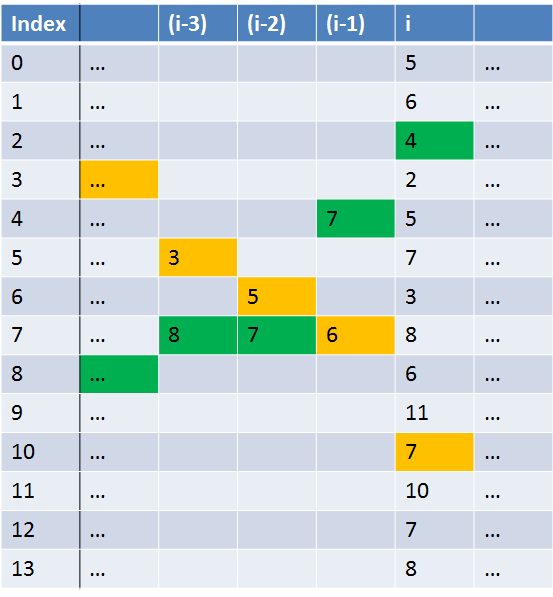
\includegraphics[width=0.75\textwidth]{4_Efficient_Toepassen_Transformatie/matrix}
  \caption{Illustratie van de \textit{matrix}-variabele. Illustratie van beste pad voor 2 verschillende toonhoogtes.}
  \label{figuur:matrix}
\end{figure}

\subsubsection{Initialisatie}
De eeste stap in het algoritme zal de noot op positie 1 als huidige noot bekijken en de noot op positie 0 als vorige noot. De hulpvariabelen moeten dus ge\"initialiseerd worden zodat ze daaraan voldoen. Hierdoor zal de array \textit{past} voor al zijn posities een hele lage waarde meekrijgen (-100 als logaritme van de probabiliteit in de broncode weergegeven in appendix \ref{Broncode:algo1}) behalve voor de noot op positie 6. Deze noot staat namelijk voor dezelfde noot als oorspronkelijke noot en aangezien de oorspronkelijke noot op positie 0 nooit getransformeerd wordt, zal \textit{past[6] = 0}. Dit betekent dat dat kans op het behouden van de eerste noot gelijk is aan 1. De \textit{current} array krijgt voor al zijn posities zeer lage waarden mee. De bedoeling hiervan is dat eender welk pad dat als eerste gevonden wordt dat voortgaat op de vorige noot een hogere probabiliteit zal hebben dan deze waarde. Tot slot zal ook elke waarde van \textit{matrix} op een arbitraire startwaarde 0 gezet worden. De waarde die hier in het begin gezet wordt is van geen belang, aangezien deze waarden toch overschreven zullen worden wanneer de beste paden berekend worden.

\subsubsection{Een stap in het algoritme}
Voor elke noot in het muziekstukje, beginnend vanaf de noot op positie 1, zal nu het volgende uitegevoerd worden. Stel ook dat we momenteel als huidige noot, de noot op positie n beschowen.\\ 
Allereerst gaan we op \textit{current[6]} de waarde zetten van het beste pad dat de huidige noot niet transformeert. Om dit te doen gaan we kijken naar de probabiliteiten van de beste paden die eindigen op alle 14 mogelijke noten die als vorige noot zouden kunnen doorgaan. Deze probabiliteiten staan uiteraard gewoon in \textit{past}. Voor elk element \textit{past[i]} wordt nu zijn waarde bij de afstandsprobabiliteit ten opzichte van de huidig beschouwde noot opgeteld. Als deze waarde hoger is dan de huidige beste waarde van \textit{current[6]}, dan wordt de waarde van \textit{current[6]} overschreven en wordt de waarde \textit{matrix[n][6]} op i gezet.
Als tweede stap gaan we voor elke mogelijk transformatie kijken naar welke noot de noot op `P+i-6' de noot huidige noot gaat afbeelden. En dit voor alle 14 mogelijke vorige noten. Stel nu dat de noot `P-i+6' de huidig beschouwde noot afbeeldt op noot `C+j-6'. Als nu de de som van \textit{past[i]} en de afstandsprobabiliteit tussen deze twee noten groter is dan de huidige waarde \textit{current[j]}, dan zal deze waarde overschreven worden. Alsook zal \textit{matrix[n][j]} gelijk gesteld worden aan i. Dit aangezien het nieuwe meest waarschijnlijke pad dat gevonden is dat eindigt op `C+j-6', komt van de noot `P+i-6'.\\
In figuur \ref{figuur:stap_algo_1} wordt een voorbeeld gegeven van de mapping van probabiliteiten horende bij noten uit de \textit{past}-array naar nieuwe probabiliteiten horende bij noten uit de \textit{current}-array. Bij deze mapping werd gebruik gemaakt van 1 transformatie die gekarakteriseerd wordt door de waarden in tabel \ref{tabel:transformatie}. In dit voorbeeld wordt ook gesteld dat de huidige noot in het originele stuk 3 halve tonen hoger lag dan de vorige noot. Met de informatie van het verschil in toonhoogte tussen de huidige en de vorige noot en de gegeven transformatie kunnen nu de verschillende sprongen bepaald worden die de huidige noot zou ondergaan, afhankelijk van welke van de 14 noten uit de \textit{past}-array als vorige noot beschouwd wordt. De pijlen geven uiteindelijk nog aan naar welke cel in de \textit{current}-array al deze sprongen zouden leiden. Een waarde in de \textit{current}-array wordt enkel aangepast wanneer er een pijl is die aankomt in deze cel, die ook nog leidt tot een hogere score dan de waarde die al in die cel staat. De score waarover gesproken wordt is de som van de waarde in de \textit{past}-array waarvan de deze pijl vertrekt en het logaritme van de afstandswaarschijnlijkheid. 
Wanneer dit uitgevoerd is, bevat \textit{current} de probabiliteiten van de beste paden van lengte (n+1) die eindigen op de 14 mogelijke toonhoogtes waarop de huidig beschouwde noot kan afgebeeld worden.
Het enige wat nu nog rest is om de waarden van \textit{current} over te zetten naar \textit{past}. En om \textit{current} daarna terug te initialiseren op zeer lager waarden. Dit zodat de arrays klaar zijn voor het beschouwen van de volgende noot in het muziekstukje. 

\begin{figure}[!ht]
  \centering
  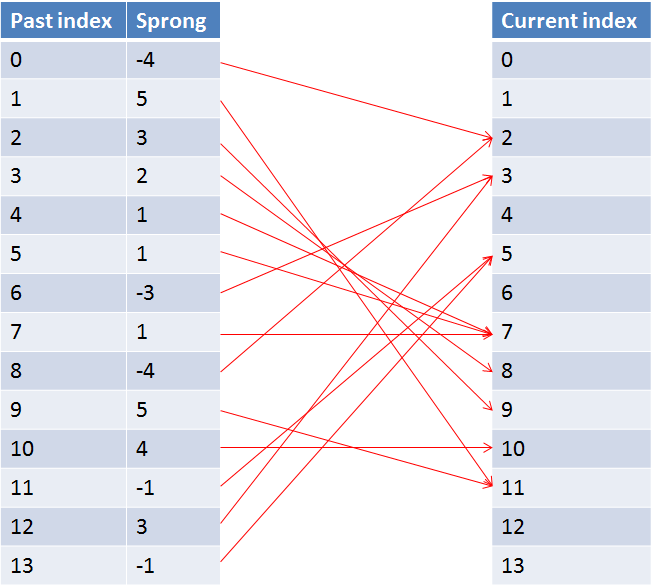
\includegraphics[width=0.75\textwidth]{4_Efficient_Toepassen_Transformatie/stap_algo_1}
  \caption{Illustratie van de \textit{past}- en \textit{current} variabelen tijdens een stap in het algoritme. De weergave is enkel voor de transformatie weergegeven in tabel \ref{tabel:transformatie}. Dit is een voorbeeld voor het specifieke geval waarin de huidige noot in het originele stuk 3 halve tonen hoger ligt dan de vorige noot.}
  \label{figuur:stap_algo_1}
\end{figure}

\begin{table}
  \centering
  \begin{tabular}{c | c  c  c  c  c  c  c  c }
    diff mod 8 & 0 & 1 & 2 & 3 & 4 & 5 & 6 & 7 \\
    \hline
    sprong & 5 & -4 & 1 & -3 & 1 & 1 & 2 & 3 \\
  \end{tabular}
  \caption{Voorstelling transformatie gebruik in figuur \ref{figuur:stap_algo_1}.}
  \label{tabel:transformatie}
\end{table}

\subsubsection{Extractie van het beste pad}
Na uitvoeren van het vorige gedeelte voor elke noot in het muziekstukje zal \textit{past} de probabiliteiten bevatten van de beste paden voor elk van de 14 mogelijke eindnoten van het geheel van het nieuwe muziekstukje. Als eerste zal er dus gekeken worden welke van deze 14 toonhoogtes het meest waarschijnlijke pad heeft. Dit pad is het pad dat we zoeken in dit algoritme. Het enige wat nu nog rest is om vanaf dit punt dat pad te reconstueren. Dit gebeurt met behulp van de \textit{matrix} array. Beginnen bij de laatste noot en zo opschuivend terug naar voor wordt hiervoor het volgende gedaan. Stel we zitten bij noot n. Noem `C+i-6' de toonhoogte van de huidige noot die in dit beste pad zit. Noem nu \textit{matrix[n][i]} = j. Dan is de vorige noot van het optimale pad de noot met als toonhoogte `P+j-6', waarbij P de toonhoogte is van de overeenkomstige noot in het originele muziekstuk. \textit{matrix[n-1][j]} geeft dan weer aanleiding tot de noot die daarvoor staat in het optimale pad, enzovoort. Op deze manier kan het volledige optimale pad weer gereconstrueerd worden. Figuur \ref{figuur:matrix} kan nogmaals als illustratie dienen voor dit principe.

\subsection{Performantie en geheugencomplexiteit}
De parameters waarvan het algoritme afhankelijk is, zijn de lengte van de melodielijn en dus het aantal noten (AN) in de invoer en ook het aantal transformaties (AT) (in het voorbeeld beschreven in appendix \ref{Broncode:algo1} wordt gebruik gemaakt van slechts 2 transformaties, maar het algoritme werkt voor eender welk aantal transformaties dat gedefini\"eerd wordt).

\subsubsection{Tijd} 
De snelheid van het algoritme is lineair afhankelijk van beide van deze parameters. Indien de lengte van het originele melodietje met een factor f omhoog gaat en de rest constant blijft dan gaat ook het aantal stappen in het algoritme met een factor f omhoog. Het rekenwerk per stap blijft echter gelijk. Wanneer het aantal transformaties met een factor f omhoog gaat en de rest constant blijft, dan zal het aantal stappen onveranderd blijven. Het rekenwerk per stap gaat wel met een factor f omhoog (op het constante rekenwerk per stap van het `niet transformeren' na).

\begin{center}
\underline{Tijd:} $\mathcal{O}(AN \times AT)$
\end{center}

\subsubsection{Geheugen}
Het geheugen dat nodig is voor de uitvoer van het algoritme is lineair afhankelijk van de lengte van de originele melodie. Dit komt omdat de \textit{matrix} array als een van zijn dimensies deze lengte heeft. Wanneer de lengte van het originele stukje met een factor f omhoog gaat, zal de grootte van deze array dus ook met een factor f omhoog gaan. De grootte van de andere twee gebruikte arrays tijdens de uitvoer van het algoritme is onveranderlijk ten opzichte van die lengte. Maar in het total geheugengebruik is de \textit{matrix} array dominant aangezien deze zo veel groter is. Het aantal gebruikte transformaties heeft geen effect op het geheugengebruik van het algoritme.

\begin{center}
\underline{Geheugen:} $\mathcal{O}(AN)$
\end{center}

\section{Beste sequentie met minimum transformatie lengte}
\label{ETT:algo2}

\subsection{Doelstelling}
Het algoritme dat in dit onderdeel beschreven wordt heeft dezelfde doelstelling als het algoritme beschreven in onderdeel \ref{ETT:algo1}. Enkel wordt dit algoritme aan nog een extra restrictie onderworpen. Zo zal dit algoritme afhankelijk zijn van drie parameters. De eerste twee parameters zijn een originele melodielijn en een aantal toegelaten transformaties. Als extra parameter is dit algoritme nog afhankelijk van een opgegeven minimum transformatie lengte. Dit betekent dat het algoritme enkel een deel van de originele melodielijn mag transformeren als hij voor minstens dit opgegeven aantal opeenvolgende noten dezelfde transformatie toepast. Er zijn een aantal overeenkomsten tussen dit algoritme en het algoritme beschreven in sectie \ref{ETT:algo1}. Bij het bespreken van deze overeenkomsten zal er verwezen worden naar overeenkomstige delen in dat hoofdstuk. Daar waar dit algoritme verschilt van het vorige zal een volledige uitleg gegeven worden.

\subsection{Idee van het algoritme}
Ook nu zal er gebruik gemaakt worden van de principes van \textit{dynamic programming}. Dit zal enkel op een verschillende manier gebeuren dan bij het vorige algoritme, aangezien de opgegeven minimumlengte verhindert om eenzelfde data representatie te gebruiken, waarom dit precies noodzakelijk is wordt verder in de tekst nog verduidelijkt. Het idee van dit algoritme bestaat erin om elke noot van het muziekstukje chronologisch te overlopen. En bij elke noot uit het originele stuk zijn er dan een aantal mogelijkheden om het beste pad te bepalen dat eindigt op een van de 14 mogelijke noten waarin de originele noot kan getransformeerd worden. Als in het vervolg van de tekst gesproken wordt over een `geldig pad', dan wordt hier een pad mee bedoeld dat de regels van de minimumlengte voor transformatie en de mogelijke transformaties respecteert. De parameter die voor de minimum transformatie lengte staat wordt met `ML' aangeduid. Een eerste mogelijkheid voor zo een optimaal pad is de uitbreiding van eender welk optimaal pad dat eindigt bij de vorige noot met het behouden van de huidige noot. Een tweede mogelijkheid is het uitbreiden van een optimaal pad dat geldig is, eindigt op de vorige noot en eindigt met transformatie f (en dus minstens zijn ML laatste noten met die transformatie is bekomen aangezien we al stelden dat het pad geldig was) uit te breiden met weer dezelfde transformatie f. Tot slot is er ook nog de mogelijkheid om eender welk optimaal en geldig pad van lengte ML korter dan het huidige uit te breiden met ML keer dezelfde transformatie. Op deze manier kunnen alle optimale paden bekomen worden die aan de vooropgestelde eisen voldoen.

\subsection{Werking van het algoritme}
In dit onderdeel zal de werking van het algoritme beschreven worden. Als extra referentie voor de lezer is de broncode bijgevoegd in appendix \ref{Broncode:algo2}.\\
Tijdens de uitvoering van het algoritme worden er 8 hulpvariabelen (allemaal arrays) gebruikt die hieronder opgelijst staan, met korte uitleg over hun betekenis.

\begin{itemize}
    \item \textbf{prob\textunderscore keep\textunderscore past:} Houdt de probabiliteiten bij voor de optimale 	en geldige paden die eindigen op een van de laatste ML bekeken noten. En dit 		enkel voor de paden die eindigen zonder transformatie van de laatste noot.
    \item \textbf{prob\textunderscore keep\textunderscore current:} Houdt de probabiliteit bij voor het optimaal en geldig pad dat eindigt op de huidig beschouwde noot. En dit enkel voor de paden die eindigen zonder transformatie van hun laatste noot.
    \item \textbf{prob\textunderscore transform\textunderscore past:} Houdt voor elke toegelaten transformatie afzonderlijk de probabiliteiten bij voor de optimale en geldige paden die eindigen met deze transformatie. En dit voor al zo een paden die eindigen op een mogelijke transformatie van een van de laatste ML beschouwde noten.
    \item \textbf{prob\textunderscore transform\textunderscore current:} Houdt voor elke toegelaten transformatie afzonderlijk de probabiliteiten bij voor de optimale en geldige paden die eindigen met deze transformatie. En dit voor al zo een paden die eindigen op de huidig beschouwde noot.
    \item \textbf{path\textunderscore end\textunderscore on\textunderscore keep\textunderscore past:} Houdt de optimale en geldige paden bij die horen bij de probabiliteiten weergegeven in \textit{prob\textunderscore keep\textunderscore past}.
    \item \textbf{path\textunderscore end\textunderscore on\textunderscore keep\textunderscore current:} Houdt het optimale pad bij dat hoort bij de probabiliteit weergegeven in \textit{prob\textunderscore keep\textunderscore current}.
    \item \textbf{prob\textunderscore end\textunderscore on\textunderscore transform\textunderscore past:} Houdt de optimale en geldige paden bij, horende bij de probabiliteiten van \textit{prob\textunderscore transform\textunderscore past}.
    \item \textbf{prob\textunderscore end\textunderscore on\textunderscore transform\textunderscore current:} Houdt de optimale en geldige paden bij, horende bij de probabiliteiten van \textit{prob\textunderscore transform\textunderscore current}.
\end{itemize}

Ter verduidelijking worden de vormen en groottes van deze variabelen visueel voorgesteld met een aantal illustraties. In figuur \ref{figuur:prob_keep_algo_2} worden de datastructuren weergegeven die betrekking hebben tot het `niet-transformeren' van de laatst beschouwde noot. In figuur \ref{figuur:prob_transform_algo_2} worden de datastructuren weergegeven die betrekking hebben tot het transformeren van de laatst beschouwde noot. Voor elke toegestande transformatie (in het totaal `AT' aantal transformaties) apart wordt er dezelfde soort info bijgehouden als voor het geval van `niet-transformatie'. In figuren \ref{figuur:path_keep_algo_2} en \ref{figuur:path_transform_algo_2} wordt weergegeven hoe de optimale (en geldige) paden bijgehouden worden die horen bij de probabiliteiten uit de vorige twee figuren. In de twee `past' tabellen uit deze twee figuren valt nog op te merken dat een pad dat rechts van een ander pad in zo een tabel staat, telkens exact een element langer is dan het andere. Dit komt omdat er voor dat optimale pad dat rechts staat al een element extra beschouwd is, dat dan al dan niet getransformeerd kan zijn.\\

Het valt op dat in dit algoritme optimale paden bijgehouden worden afhankelijk van met welke specifieke transformtie hun laatste noot bekomen is. Dit in tegenstelling tot het vorige algoritme waar er een gemeenschappelijke \textit{matrix} werd opgesteld waaruit het optimale pad later geconstrueerd kon worden. De reden dat zo een matrix wel werke in het vorige algoritme was precies omdat er geen eis van minimum lengte was voor een transformatie. Dit betekent dat voor eender welke noot, er kan besloten worden enkel afgaande op de probabiliteiten van de mogelijke toonhoogtes die de vorige noot kan aannemen, wat de probabiliteiten zijn van de toonhoogtes waarnaar de huidige noot getransformeerd kan worden. Stel nu dat we voor het algoritme besproken in dit onderdeel, dezelfde voorstelling zouden willen gebruiken. Dan zijn er twee problemen waar we op botsen. Ten eerste, als we willen transformeren moet dat voor minsten ML opeenvolgende noten zijn, het volstaat dus niet meer om gewoon naar de vorige laag te kijken in de matrix om de nieuwe te bepalen, we gaan ook ML eenheden verder moeten teruggaan om op suboplossingen die voldoende korter zijn ineens ML keer de transformatie toe te passen. Het volgende probleem is dat we zelfs als we dan een nieuw pad vinden, we dit (voorlopig) optimale pad niet zomaar kunnen inschrijven in de \textit{matrix}, aangezien we dan ook andere paden zouden kunnen aanpassen die daardoor mogelijks een deel van hun pad getransformeerd zouden zien over een lengte korter dan ML. 

\begin{figure}[!ht]
  \centering
  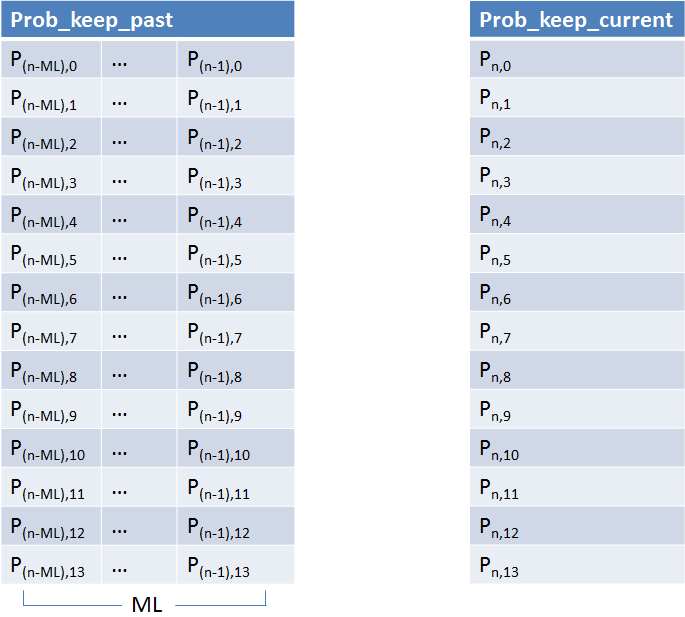
\includegraphics[width=0.75\textwidth]{4_Efficient_Toepassen_Transformatie/prob_keep_algo_2}
  \caption{Illustratie van de variabelen die probabiliteiten opslaan met betrekking tot het `niet-transformeren' van de laatste noot. Elk element in deze tabel stelt een (logaritme van een) probabiliteit voor.}
  \label{figuur:prob_keep_algo_2}
\end{figure}

\begin{figure}[!ht]
  \centering
  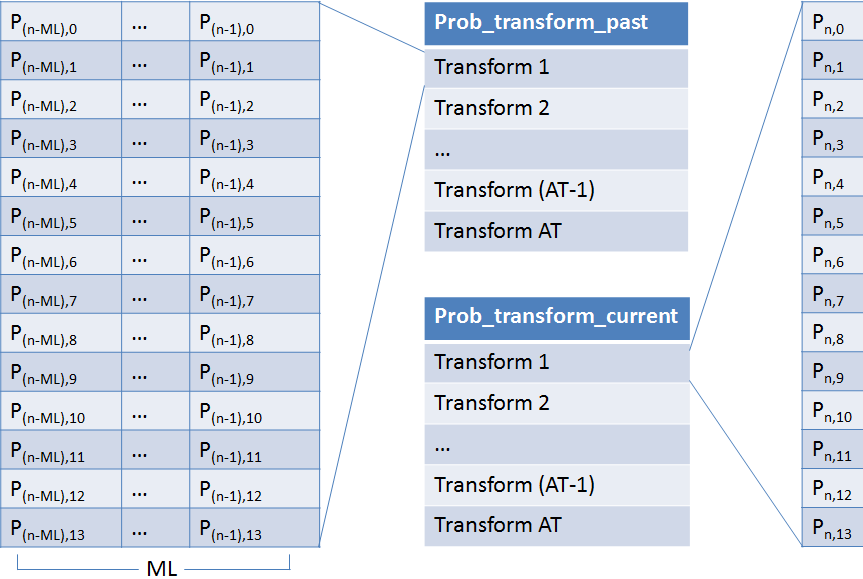
\includegraphics[width=0.75\textwidth]{4_Efficient_Toepassen_Transformatie/prob_transform_algo_2}
  \caption{Illustratie van de variabelen die probabiliteiten opslaan met betrekking tot het transformeren van de laatste noot. Elk element in deze tabel stelt een (logaritme van een) probabiliteit voor.}
  \label{figuur:prob_transform_algo_2}
\end{figure}

\begin{figure}[!ht]
  \centering
  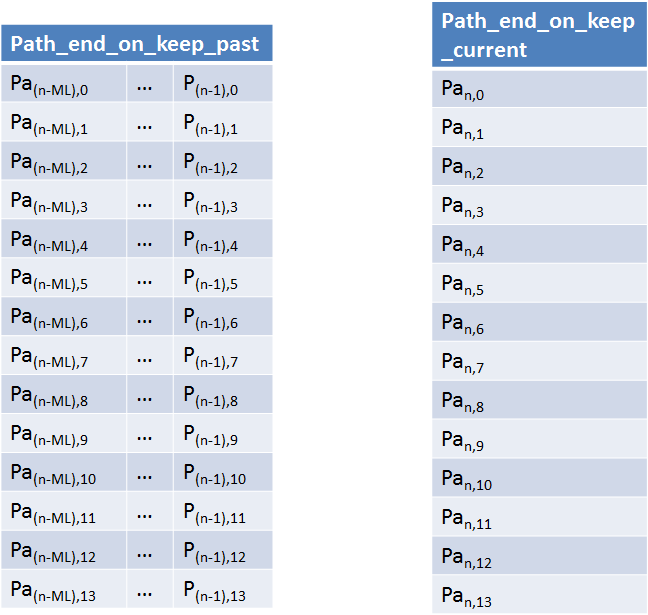
\includegraphics[width=0.75\textwidth]{4_Efficient_Toepassen_Transformatie/path_keep_algo_2}
  \caption{Illustratie van de variabelen die optimale (geldige) paden opslaan met betrekking tot het `niet-transformeren' van de laatste noot. Elk element in deze tabel stelt een optimaal en geldig pad voor.}
  \label{figuur:path_keep_algo_2}
\end{figure}

\begin{figure}[!ht]
  \centering
  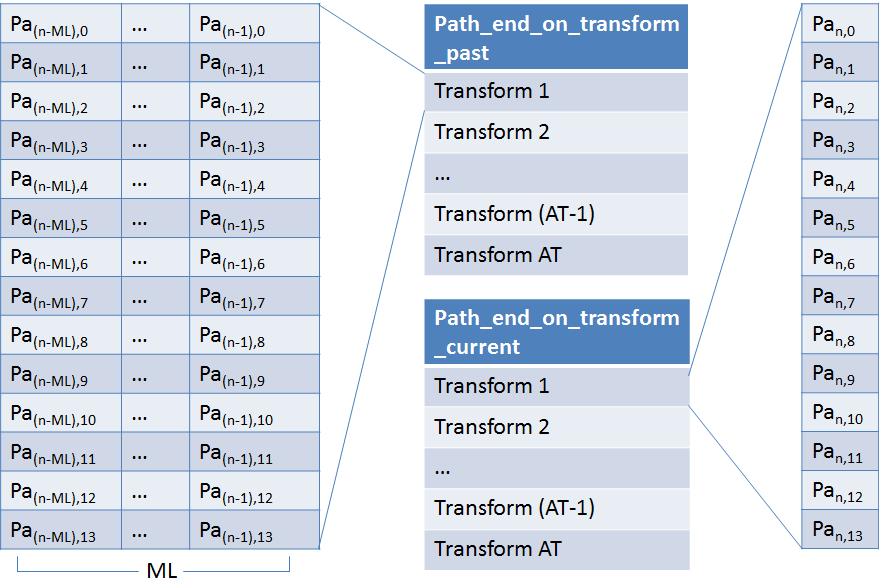
\includegraphics[width=0.75\textwidth]{4_Efficient_Toepassen_Transformatie/path_transform_algo_2}
  \caption{Illustratie van de variabelen die optimale (geldige) paden opslaan met betrekking tot het transformeren van de laatste noot. Elk element in deze tabel stelt een optimaal en geldig pad voor.}
  \label{figuur:path_transform_algo_2}
\end{figure}

\subsubsection{Initialisatie}
De initialisatie verloopt vrij eenvoudig. Alle variabelen die optimale paden bijhouden worden ge\"initialiseerd op een lege array. Aangezien er voor de uitvoer van het algoritme uiteraard nog geen deel van een pad berekend is. De variabelen die betrekking hebben op de probabiliteiten van de optimale paden worden allemaal op een zeer lage waarde ge\"initialiseerd. Dit behalve voor variabele \textit{prob\textunderscore keep\textunderscore past}, waarvan de waarde horende bij de probabiliteit op het behouden van de eerste noot op 0 wordt gezet (wat overeenkomt met een kans van 1 aangezien de waarden waarmee gerekend wordt, de logaritmen zijn van de eigenlijke waarden). Dit omdat de eerste noot van een melodielijn altijd behouden wordt, want om een transformatie in rekening te brengen moet er een vorige noot zijn die niet bestaat voor de eerste noot.

\subsubsection{Een stap in het algoritme}
Elke stap in het algoritme komt overeen met het berekenen voor de optimale paden van het algoritme voor de melodielijn die een noot meer van het originele stuk bevat dan in de vorige stap. Om deze optimale paden te berekenen wordt gebruik gemaakt van de optimale paden van de vorige stappen in het algoritme. Deze worden dan zo effici\"ent mogelijk uitgebreid tot aan de huidig beschouwde noot. In de rest van deze paragraaf wordt er vanuit gegaan dat we momenteel bij noot n in het muziekstuk zitten in het algoritme. En we zoeken nu dus de optimale paden voor het toepassen van het algoritme op de eerste n+1 noten (aangezien de eerste noot, noot 0 is).\\
Een eerste mogelijkheid om een optimaal pad te vinden van n+1 noten is om een van de optimale paden van lengte n uit te breiden met een `niet-transformatie' door de noot op positie n in het oorspronkelijk melodie gewoon te behouden. In dit geval maakt het niet uit of zo een optimaal pad van lengte n eindigt op een specifieke transformatie of niet. Indien zo een nieuw pad een hogere waarschijnlijkheid heeft dan het beste pad tot nu toe dan wordt dit pad opgeslagen in \textit{path\textunderscore end\textunderscore on\textunderscore keep\textunderscore current} en de overeenkomstige probabiliteit wordt bijgehouden in \textit{prob\textunderscore keep\textunderscore current}.\\
Een tweede mogelijkheid is om een nieuw pad van lengte n+1 te construeren dat eindigt om een van de toegelaten transformaties. Voor elke transformatie f kan er dan het volgende gedaan worden op mogelijke optimale paden te vinden. Er is een eerste mogelijkheid om een optimaal pad van lengte n dat al eindigde op dezelfde transformatie uit te breiden naar een pad van lengte n+1 met deze transformatie. Er is nog een tweede mogelijkheid waarbij een optimaal pad van lengte n+1-ML wordt uitgebreid met ML transformaties volgens transformatie f. Dit om te voldoen aan de eisen van de minimum lengte van een transformatie. Deze paden van lengte n+1-ML waarover gesproken wordt kunnen zowel eindigen op een van de andere transformaties als te eindigen op een `niet-transformatie'. Zolang ze daarna maar uitgebreid worden met ML keer de transformatie f. Ook hier zal bij al deze combinaties gekeken worden op de probabiliteit van het nieuwe geconstrueerde pad hoger ligt dan het beste pad tot nu toe. Indien dit het geval is wordt dit nieuwe pad opgeslagen in \textit{path\textunderscore end\textunderscore on\textunderscore transform\textunderscore current} en de overeenkomstige probabiliteit wordt bijgehouden in \textit{prob\textunderscore transform\textunderscore current}.\\
Als laatste gedeelte van elke stap van het algoritme worden, net zoals in het algoritme beschreven in de vorige sectie, de variabelen weer klaargemaakt voor de uitvoer van de volgende iteratie. Alle probabiliteiten en paden worden een tijdsstap doorgeschoven in hun overeenkomstige variabelen. Paden die meer dan ML korter zijn dan de huidige beschouwde lengte worden niet meer bijgehouden. Dus voor elke iteratie n zullen aan het eind van de iteratiestap alle paden met lengte n+1-ML verwijderd worden omdat ze niet meer noodzakelijk zijn voor het vervolg van het algoritme.

\subsubsection{Extractie van het beste pad}
In tegenstelling tot het vorige algoritme waar het optimale pad nog moest bepaald worden door terug te lopen door de \textit{matrix}, zal de extractie van het optimale pad na uitvoeren van het algoritme hier een stuk vlotter verlopen. Dit komt doordat de volledige optimale paden van de deelproblemen (en uiteindelijk dus ook van het gehele probleem) telkens opgeslagen worden in hulpvariabelen. Het enige wat moet gebeuren om het beste pad te vinden is dus kijken naar alle mogelijke optimale paden voor de volledige melodie. Voor elke mogelijke transformatie en voor elke mogelijke eindnoot die met deze transformatie kan bekomen worden gaan we zo een optimaal pad hebben. En van deze optimale paden gaat het pad gekozen worden met de hoogste waarschijnlijkheid. Dit pad is het gezochte optimale pad dat voldoet aan alle voorwaarden opgelegd aan het algoritme.

\subsection{Performantie en geheugencomplexiteit}
In dit algoritme zijn er drie parameters waar rekening mee dient gehouden te worden bij het bespreken van de tijds- en geheugencomplexiteit. Deze drie parameters zijn het aantal noten in de originele melodielijn (AN), het aantal beschikbare transformaties (AT) en de minimum transformatie lengte (ML).

\subsubsection{Tijd}
De performantie van het algoritme is lineair afhankelijk van het aantal noten. Dit komt doordat voor elke noot in het oorspronkelijk muziekstuk een stap in het algoritme moet uitgevoerd worden, het rekenwerk per stap verandert niet wanneer de lengte van het stuk verandert. De snelheid van het algoritme is kwadratisch afhankelijk van het aantal toegestane transformaties. Dit komt omdat voor elke stap in het algoritme we voor elke transformatie gaan proberen een optimaal pad te vinden dat kan vertrekken van bij tussenoplossingen horende bij alle andere transformaties. Het aantal stappen in het algoritme verandert niet wanneer het aantal transformaties verandert. In totaal geeft dit dus een kwadratische afhankelijkheid. Tot slot is de snelheid van het algoritme ook afhankelijk van de minimum transformatie lengte volgens $\mathcal{O}(ML \times (AN-ML))$. zowel het aantal stappen in het algoritme als het aantal berekende paden per stap zal onveranderd blijven wanneer deze parameter verandert. Het extra rekenwerk dat gecre\"eerd wordt door het moeten uitbreiden van paden die ML korter zijn dan de huidige lengte is lineair afhankelijk van de grootte van ML. Maar het aantal paden dat zo berekend moet worden is lineair afhankelijk van (L-ML). Hierdoor zal de totale rekentijd afhankelijk zijn van het product van deze twee.

\begin{center}
\underline{Tijd:} $\mathcal{O}(AN \times ML \times (AN-ML) \times AT^2)$
\end{center}

\subsubsection{Geheugen}
De totale opslagcapaciteit die noodzakelijk is voor de uitvoer van het algoritme is ten eerste lineair afhankelijk van de lengte van de invoersequentie van noten. Voor alle mogelijke transformaties zullen namelijk optimale paden bijgehouden worden en de lengte va, deze paden is altijd van dezelfde grootte-orde als de lengte van het originele. Ten tweede is het geheugengebruik ook lineair afhankelijk van de minimum transformatie lengte. Er worden namelijk optimale sub paden bijgehouden in het algoritme voor de laatste ML beschouwde noten. De lengte van deze paden is ook elk van dezelfde grootte-orde. Tot slot is er nog het aantal transformaties. Ook deze parameter zal een lineaire invloed hebben op het geheugengebruik. Dit aangezien voor elke toegestane transformatie even veel optimale paden bijgehouden worden die eindigen op die zelfde transformatie.  

\begin{center}
\underline{Geheugen:} $\mathcal{O}(AN \times ML \times AT)$
\end{center}

%%% Local Variables: 
%%% mode: latex
%%% TeX-master: "masterproef"
%%% End: 
